\documentclass[
  english,            % define the document language (english, german)
  aspectratio=169,    % define the aspect ratio (169, 43)
  % handout=2on1,       % create handout with multiple slides (2on1, 4on1)
  % partpage=false,     % insert page at beginning of parts (true, false)
  % sectionpage=true,   % insert page at beginning of sections (true, false)
]{tumbeamer}


% load additional packages
\usepackage{booktabs}
\usepackage{amssymb}
\usepackage{mdframed}
\usepackage{amsthm}
\usepackage{mathtools}
\usepackage{multicol}
\usepackage{hyperref}
\usepackage{caption}
%\usepackage{julialogo}

\usepackage{biblatex}
\renewcommand*{\bibfont}{\normalfont\small}
\addbibresource{juliacon_GAIO.bib}

\makeatletter
\patchcmd{\@Aboxed}{\boxed{#1#2}}{\fcolorbox{white}{blue!20}{$\displaystyle #1#2$}}{}{}%
\makeatother

\newtheorem{theorem}{Theorem}
\newtheorem{lemma}{Lemma}
\newtheorem{definition}{Definition}
\newtheorem{proposition}{Proposition}

%\usepackage{courier}
\usepackage{xcolor}
\usepackage{tikz}
\usepackage{tikzit}
\usetikzlibrary{shapes,arrows,calc,decorations.pathreplacing,angles,quotes}

\input{colors.tikzstyles}

\usepackage{empheq}
\usepackage{tcolorbox}

\tcbset{highlight math style={colback=blue!20!white,arc=2pt,boxrule=0pt}}
\newenvironment{emphbox}
  {\begin{tcolorbox}[colback=blue!5!white,colframe=blue!75!black]}
  {\end{tcolorbox}}


\usepackage{algpseudocodex}
\usepackage{algorithm}

%\colorlet{lightblue}{!10}
\usepackage{listings}
\lstset{
	basicstyle=\ttfamily,
	backgroundcolor = \color{blue!10},
	keywordstyle=\color{blue},
    numberstyle=\tiny\color{codegray},
    stringstyle=\color{purple},
    basicstyle=\ttfamily\footnotesize,
	% numbers=left, 
	numberstyle={\footnotesize \color{blue!50}},
	xleftmargin=.1in,
	numbersep=3pt,
	literate={\$}{{\textcolor{blue}{\$}}}1,
  showlines=true 
}
	
\usepackage{lmodern}

\usepackage{fontawesome}
\usepackage{julialogo}

\usepackage{nameref}
\makeatletter
\newcommand*{\currentname}{\@currentlabelname}
\makeatother
%\usepackage{dsfont}

\newcommand{\R}{{\mathbb R}}
\newcommand{\N}{{\mathbb N}}
\newcommand{\E}{{\mathbb E}}
\renewcommand{\P}{{\mathbb P}}
\newcommand{\bbC}{{\mathbb C}}
\newcommand{\cO}{\mathcal{O}}
\newcommand{\cF}{\mathcal{F}}
\newcommand{\cE}{\mathcal{E}}
\newcommand{\cX}{\mathcal{X}}
\newcommand{\cA}{\mathcal{A}}
\newcommand{\cS}{\mathcal{S}}
\newcommand{\cR}{\mathcal{R}}
\newcommand{\cB}{\mathcal{B}}
\newcommand{\cP}{\mathcal{P}}

\newcommand{\tV}{\widetilde{V}}
\newcommand{\tF}{\widetilde{F}}
\newcommand{\tQ}{\widetilde{Q}}

\newcommand{\bw}{\mathbold{w}}

\newcommand{\step}[1]{\mathds{1}_{\{#1\ge 0\}}}

\newcommand{\eps}{\varepsilon}

\renewcommand{\emph}[1]{\textcolor{purple}{#1}}
\newcommand{\argmax}{\mathop{\textrm{argmax}}}
\newcommand{\mean}{\mathop{\textrm{mean}}}
\newcommand{\diam}{\mathop{\textrm{diam}}}


\setbeamertemplate{itemize items}[circle]

% presentation metadata
\title{Fast, Set-Oriented Numerical Analysis using GAIO.jl}
\author{April Herwig}

\institute{\theChairName\\\theDepartmentName\\\theUniversityName}
\date{}

%\footline{\insertauthor~|~\insertshorttitle~|~\insertshortdate}
\footline{}


% macro to configure the style of the presentation
\TUMbeamersetup{
  title page = TUM centered,         % style of the title page
  part page = TUM toc,            % style of part pages
  section page = TUM toc,         % style of section pages
  content page = TUM more space,  % style of normal content pages
  tower scale = 1.0,              % scaling factor of TUM tower (if used)
  headline = TUM empty,      % which variation of headline to use
  footline = TUM default,         % which variation of footline to use
  % configure on which pages headlines and footlines should be printed
  headline on = {title page},
  footline on = {every page, title page=false},
}

% available frame styles for title page, part page, and section page:
% TUM default, TUM tower, TUM centered,
% TUM blue default, TUM blue tower, TUM blue centered,
% TUM shaded default, TUM shaded tower, TUM shaded centered,
% TUM flags
%
% additional frame styles for part page and section page:
% TUM toc
%
% available frame styles for content pages:
% TUM default, TUM more space
%
% available headline options:
% TUM empty, TUM oneliner, TUM twoliner, TUM threeliner, TUM logothreeliner
%
% available footline options:
% TUM empty, TUM default, TUM infoline

\setlength{\parskip}{1em}

\usepackage{mathpple}
%\usepackage{euler}
%\usepackage{palatino}

\begin{document}

\tikzstyle{block} = [thick, draw, rectangle, rounded corners, fill=blue!20,
                       minimum height=3em, minimum width=6em]
\tikzstyle{node} = [thick, draw, circle, fill=blue!20]
\tikzstyle{action} = [thick, draw, circle, fill=red!10]

\maketitle

\begin{frame}{Dynamical systems}

Consider a continuous map
\[
f:\R^d\to \R^d.
\] 

The map defines a \emph{discrete dynamical system} by iteration:
\[
x_{k+1} = f(x_k), \qquad k=0,1,2,\ldots
\]

\begin{tcolorbox}[colback=blue!5!white,colframe=blue!75!black]
Basic question: \textit{What is the fate of some $x_0$ as $k\to\infty$?}
\end{tcolorbox}



\end{frame}

\begin{frame}{Motivation}{Attractors}

\begin{definition}
    An invariant set $A$ is \emph{attracting} if there is a neighborhood $U$ of $A$ such that for every open set $V\supset A$ there is $K\in\N$ such that
    \[
    f^k(U)\subset V \quad\text{for all } k\ge K.
    \]
\end{definition}

\begin{proposition}
    If $A$ is a closed attracting set then
    \[
    A = \bigcap_{k\in\N} f^k(U).
    \]
\end{proposition}

\begin{emphbox}
    \textbf{Basic idea:} Successively refine an approximation of $A$ using \emph{subdivision}
\end{emphbox}

\end{frame}

\begin{frame}{Computing Attractors}{The subdivision algorithm}

Generate a sequence $\cB_0,\cB_1,\cB_2,\ldots$ of finite families of compact sets as follows:

Let $\cB_0=\{Q\}$, $\theta \in (0,1)$. For $k=1,2,\ldots$ do
\begin{itemize}
    \item construct $\hat\cB_k$ such that
    \[
    |\hat\cB_k| = |\cB_{k-1}|
    \quad\text{and}\quad \diam\hat\cB_k \leq \theta \cdot \diam\cB_{k-1}.
    \]
    \item set
    \begin{gather*}
    \cB_k = f(\hat\cB_k) \cap \hat\cB_k, \quad \text{where}\quad \\ 
    f(\hat\cB_k) \cap \hat\cB_k \,\overset{def}{=}\, \{ B\in\hat\cB_k \mid \exists B'\in\hat\cB_k: f(B')\cap B \neq \varnothing\}.
    \end{gather*}
\end{itemize}

\medskip

\begin{emphbox}
  \begin{theorem}
    $|\cB_k|\to A$ as $k\to\infty$ in the Hausdorff metric.
  \end{theorem}
\end{emphbox}

\end{frame}

\begin{frame}{Computing Attractors}{The subdivision algorithm}
  
\begin{figure}
  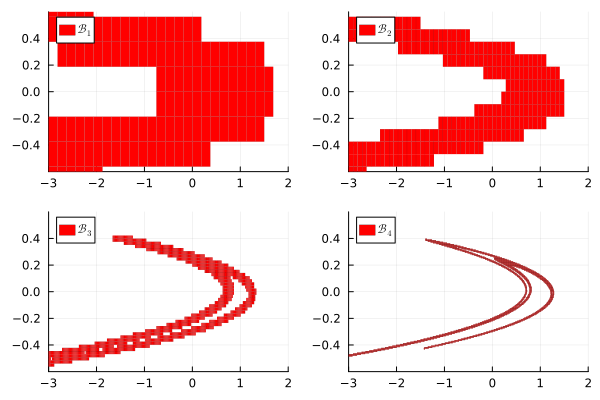
\includegraphics[height=0.8\textheight]{figures/henon_subdivisions}
\end{figure}

\end{frame}

\begin{frame}[fragile]
\frametitle{Representation of Cubical Sets}

Simple idea: partition the domain into equally sized grid of hypercubes

\begin{lstlisting}[language=Matlab,mathescape]
  $\text{\textcolor{blue}{\texttt{struct}}}$ Box{N, T}
    center::SVector{N, T}
    radius::SVector{N, T}
  end

  $\text{\textcolor{blue}{\texttt{struct}}}$ BoxPartition{B <: Box}
    domain::B
    $\text{\textcolor{black}{\texttt{size}}}$::CartesianIndex{N}
  end

  $\text{\textcolor{blue}{\texttt{struct}}}$ BoxSet{P <: BoxPartition, S <: AbstractSet{<:CartesianIndex}}
    partition::P
    cartesian_indices::S
  end
\end{lstlisting}



\end{frame}

\begin{frame}[fragile]
\frametitle{Representation of Cubical Sets}

We can use the built-in set data types and setwise operations for \texttt{BoxSet}s using \emph{multiple-dispatch}

\begin{lstlisting}[language=Matlab,mathescape]
  function Base.$\subseteq$( B$_1$::BoxSet, B$_2$::BoxSet )
    B$_1$.partition == B$_2$.partition  && 
      B$_1$.cartesian_indices $\subseteq$ B$_2$.cartesian_indices
  end

  function Base.rand( B::Box{N,T} ) where {N,T}
    c = B.center;  r = B.radius
    c .+ r .* rand(-1:eps(T):1, N)
  end
\end{lstlisting}

Combined with \texttt{BoxSet}, the \texttt{BoxPartition} serves as a $\sigma$-algebra over the domain. We can generate sets with \texttt{cover}:

\begin{lstlisting}[language=Matlab,mathescape]
  $\text{\textcolor{blue}{\texttt{cover}}}$(partition, points),   $\text{\textcolor{blue}{\texttt{cover}}}$(partition, other_boxset)
\end{lstlisting}

\end{frame}

\begin{frame}{Cell Mapping}

So how do we compute 
\[
  f(\cB) = \{ B\in\cP \mid \exists B'\in\cB: f(B')\cap B \neq \varnothing\}\ ?
\]

\begin{figure}
  \ctikzfig{boximage}
  %\caption{Image of the simple box set $\cB = \left\{ B \right\}$}
  \label{fig:boximage}
\end{figure}

\end{frame}

\begin{frame}[fragile]
\frametitle{Cell Mapping}
\framesubtitle{test point sampling}

\medskip

\begin{lstlisting}[language=Matlab,mathescape]
  function map_boxes(f, source::BoxSet; n_samples)

    B() = $\text{\textcolor{blue}{\texttt{empty}}}$(source)                    # Initialize empty BoxSet
    P = source.partition

    $\text{\textcolor{blue}{\texttt{@floop}}}$ for box in source
      for k = 1:n_samples
        p = rand(box)                 # Generate sample point
        image_p = f(p)
        hit = $\text{\textcolor{blue}{\texttt{cover}}}$(P, image_p)            # Box in P covering the point fp
        $\text{\textcolor{blue}{\texttt{@reduce}}}$($\text{\textcolor{black}{\texttt{image}}}$ = B() $\cup$ hit) $\quad\ \ \,$     # Each thread collects hits,
      end                             # after loop completion the 
    end                               # result is reduced by $\cup$

    return $\text{\textcolor{black}{\texttt{image}}}$
  end 
\end{lstlisting}

\end{frame}

\begin{frame}{Cell Mapping}{test point sampling}
  
\begin{itemize}
  \item predefine test points and (affine) transform them to $B \in \cB$ as needed
  \item memory-efficient "lazy" test point sampling with \texttt{Generator}s
  \item ensure type-stability with \texttt{FunctionWrappers} to shorten generated llvm
  \item spread load across multiple compute threads using \textcolor{blue}{\texttt{@floop}} macro
  \item collect hits and reduce per-thread result into single result using \textcolor{blue}{\texttt{@reduce}} macro
  \item "embarrasingly parallel" - can harness the GPU using CUDA.jl
\end{itemize}

\end{frame}

\begin{frame}[fragile]
\frametitle{Usage: Constructing an Attractor algorithm}

%\medskip

Compare the pseudocode algorithm

\begin{algorithmic}[1]
    %\Function{relative_attractor}{$f$, $\cB$, steps}
    \Require $f,\,\ \cB_0,\,\ n_{\text{steps}}$
    %\State $\mathcal{B}_0 \gets \mathcal{B}$

    \For{$k = \left\{ 1,\ \dotsc,\ n_{\text{steps}} \right\}$}
        %\Comment{$n$ is a predefined number of iteration steps}
        \State $\mathcal{B}_k \gets$ \Call{subdivide}{$\,\mathcal{B}_{k-1}\,$}
        \State $\mathcal{B}_k \gets \mathcal{B}_k\, \cap\, f (\,\mathcal{B}_k\,)$
    \EndFor

    \State \Return $\mathcal{B}_n$ 
    %\EndFunction
\end{algorithmic}

to the julia implementation

\begin{lstlisting}[language=Matlab,mathescape]
  function relative_attractor(F::BoxMap, $\cB$::BoxSet, steps)
    for k = 1:steps
      $\cB$ = subdivide($\cB$)
      $\cB$ = $\cB$ $\cap$ F($\cB$)
    end
    return $\cB$
  end
\end{lstlisting}

\end{frame}

\begin{frame}%[shrink=1]

\begin{figure}
  \centering
  
\includegraphics[width=0.18\textwidth]{qr-code.png}
  {\caption*{github.com/gaioguys/GAIO.jl}}
\end{figure}

\nocite{*}
\printbibliography

\end{frame}


\end{document}
